
\section{METHODOLOGY}


\subsubsection{Software Development Life Cycle}
For the study of research methods, or, more formally, ‘a contextual framework' for
research of this project, spiral model was chosen among all others as it enables
gradual releases and refinement of a product through each phase of the spiral as
well as the ability to build prototypes at each phase. Spiral model is one of the most
important Software Development Life Cycle models, which provides support
for Risk Handling. It has four phases: Planning, Design, Construct and Evaluation.
A software project repeatedly passes through these phases in iterations (called
Spirals in this model) as shown in the figure below. The Radius of the spiral at any
point represents the expenses (cost) of the project so far, and the angular
dimension represents the progress made so far in the current phase. In each phase
of the Spiral Model, the features of the product dated and analyzed, and the risks
at that point in time are identified and are resolved through prototyping.
\begin{figure}[h]
    \centering
    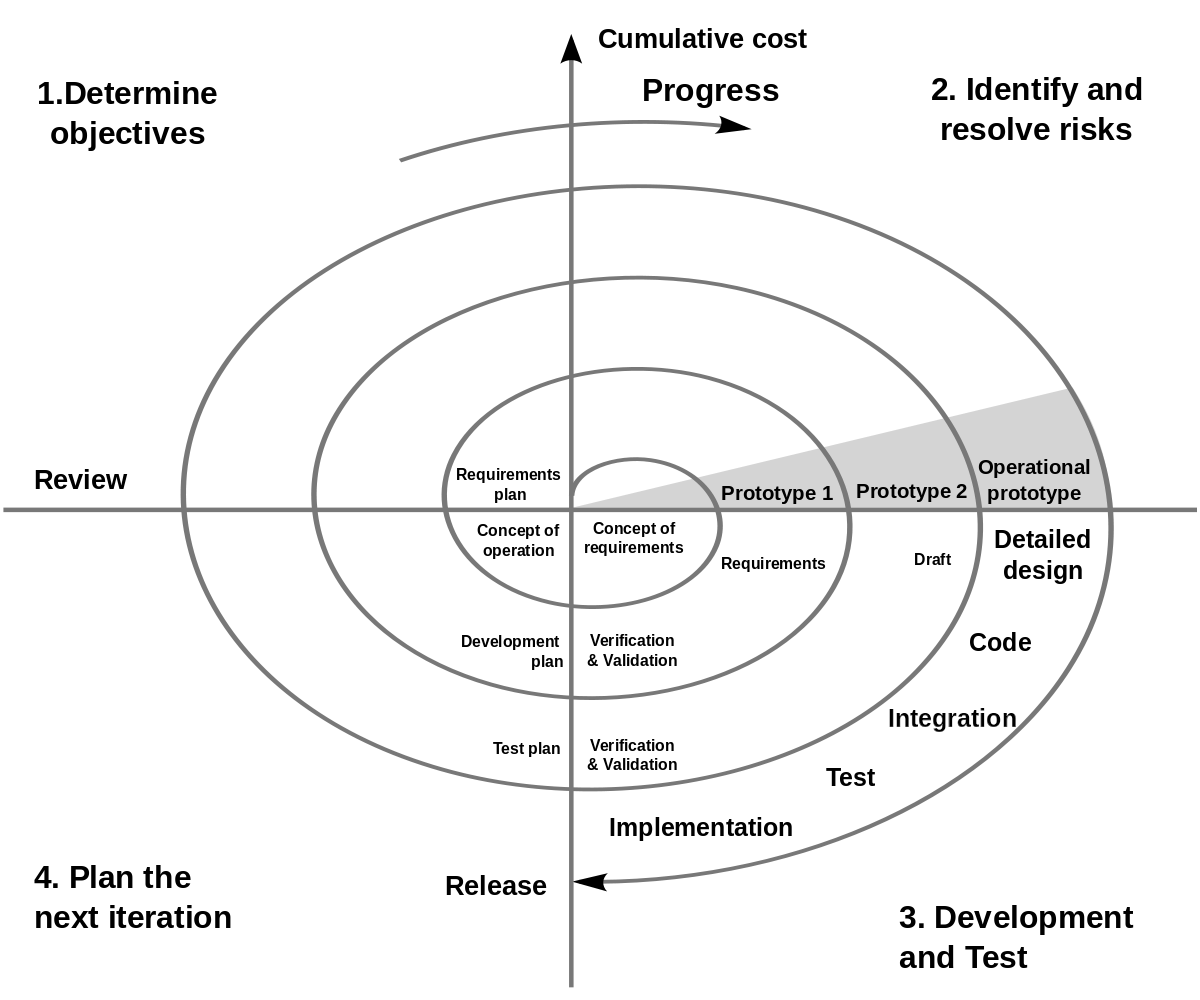
\includegraphics[width=120mm]{spiral.png}
    \caption{Spiral Model of Software Development}
    \label{fig:Spiral Model}
\end{figure}
\begin{itemize}
    \item \textbf{Planning Phase}\\
Requirements are gathered from the customers and the objectives are
identified, elaborated, and analyzed at the start of every phase. Then
alternative solutions possible for the phase are proposed in this quadrant.
     \item \textbf{Risk Analysis Phase}\\
     During the second quadrant, all the possible solutions are evaluated to
select the best possible solution. Then the risks associated with that
solution are identified and the risks are resolved using the best possible
strategy. At the end of this quadrant, the Prototype is built for the best
possible solution.
     
      \item \textbf{Development and Testing Phase}\\
      During the third quadrant, the identified features are developed and
verified through testing. At the end of the third quadrant, the next version
of the software is available.
       \item \textbf{Evaluation and Planning next Phase}\\
       In the fourth quadrant, the Customers evaluate the so far developed version
of the software. In the end, if the Customers are satisfied with the software,
then, it is released, else, planning for the next phase is started.
       
\end{itemize}


\vspace{0.5in}
\subsubsection{System Development Tools}
\begin{itemize}
    \item \textbf{MongoDB (Database)}\\
    MongoDB serves as the foundational database, storing essential user data, task details, journal entries, and digital detox preferences. Its flexible schema allows us to adapt the data model as the app evolves, ensuring efficient data management.
 
    \item \textbf{Express.js (Backend)}\\
    Express.js provides a robust backend framework, handling HTTP requests and responses, routing, middleware, and interacting with the database. This framework enables efficient server-side logic, ensuring smooth data flow between the frontend and the database.

    \item \textbf{React (Frontend)}\\
     React forms the heart of our frontend development, offering a component-based architecture for building interactive user interfaces. Its fast rendering and reusable components enable a seamless user experience while managing tasks, reflecting, and engaging with digital detox features.
     
    \item \textbf{Node.js (Runtime Environment)}\\
    Node.js serves as the runtime environment for the backend, allowing us to use JavaScript on the server-side. This enables consistent code throughout the stack and leverages the extensive Node.js package ecosystem, enhancing development efficiency.
    
     \item \textbf{Git and GitHub (Version Control and Collaboration)}
      Git enables efficient version control, allowing our development team to track changes, collaborate seamlessly, and manage different code branches effectively. We utilize GitHub as a remote repository to host our project's source code, enabling version history tracking, code review, and easy collaboration among team members. This setup ensures a structured and collaborative approach to development, making it easier to manage code changes, review contributions, and maintain a reliable and up-to-date codebase for the "Rental Room Finder" app.
\end{itemize}

